\chapter{مفاهیم اولیه}
\newpage
‎\renewcommand{\baselinestretch}{2}\normalsize‎
\label{Basic concepts}
برای درک بهتر مطالب در فصل‌های آتی رساله، در این فصل مفاهیم اولیه مورد نیاز شبکه‌های تطبیقی توزیع‌شده، انواع مدل‌های محاسباتی پردازش موازی و تاریخچه و برتری‌های مدل محاسباتی موازی‌سازی مانعی ارائه می‌گردد. 


\section{شبکه‌های تطبیقی توزیع‌شده}
معماری متمرکز و غیرمتمرکز  (توزیع‌شده) دو معماری مهم در شبکه‌ای از گره‌ها می‌باشند. در شبکه‌های متمرکز\footnote{\lr{Centralized Network}} ، به منظور تخمین پارامترها، همه گره‌ها تخمین خود را به گره مرکزی ارسال می‌نمایند. گره ‌مرکزی (سرور پارامتری) همه اطلاعات ارسال شده را تلفیق و پردازش می‌نماید. این معماری، منابع سیستم همانند زمان و پهنای باند را هدر می‌دهد و با مشکلات امنیتی و حریم خصوصی داده روبه‌رو است. همچنین اگر گره مرکزی از کار بیفتد، سیستم با شکست مواجه خواهد شد. در شبکه‌های غیرمتمرکز\footnote{\lr{Decentralized Network}} یا‌ توزیع‌شده هیچ مرکز تلفیقی وجود ندارد و این امر سبب کاهش سربارهای ارتباطی و پردازشی خواهد شد \cite{Sayed2013}. از این‌رو استراتژی‌های غیرمتمرکز بر روی شبکه‌ها کاربرد فراوانی دارند. 

با پیشرفت سریع فناوری‌های شبکه‌ای و ارتباطی، شبکه‌های توزیع‌شده‌ای که رایانه‌های شخصی، تلفن‌های همراه، حسگرها و محرک‌ها را به هم متصل می‌کنند، چهارچوب اصلی شبکه‌های ارتباطی و کنترل داده‌ را تشکیل می‌دهند. پردازش توزیع‌شده با استخراج اطلاعات از داده‌های جمع‌آوری شده در گره‌هایی که در یک منطقه جغرافیایی توزیع شده‌اند، سروکار دارد. به عنوان مثال، هر گره در یک شبکه داده‌های مربوط به یک پارامتر خاص را جمع آوری کرده و سپس برای رسیدن به برآورد پارامتر به روش خاصی و براساس توپولوژی شبکه با دیگر گره‌ها تعامل می‌کند. هدف این است که به برآوردی برسیم که دقیقاً همان نتیجه‌ای باشد که در صورت دسترسی هر گره به اطلاعات کل شبکه، بدست خواهد آمد \cite{Sayed2013}.  

شبکه‌های تطبیقی توزیع‌شده مجموعه‌ای از فیلترهای وفقی می‌باشند که برای پاسخ‌دهی به جریان داده‌های ورودی با یکدیگر ارتباط و همکاری دارند. معمولا از گراف برای نمایش آن‌ها استفاده می‌شود و هر گره خود یک فیلتر وفقی است. فیلتر وفقی استفاده شده در هر گره می‌تواند یکی از انواع فیلترهای وفقی \lr{LMS} (\lr{Least Mean Squares}) و یا \lr{RLS} (\lr{Recursive Least Squaress}) باشد. این شبکه‌ها در محیط‌های ایستان  \footnote{\lr{Stationary environment}} و غیرایستان\footnote{\lr{Non-stationary environment}}  کاربرد دارند و معمولا به‌صورت یک مسئله بهینه‌سازی با هدف بدست آوردن بردار پارامترهای مجهول با توجه به داده‌هایی که در گره‌های مختلف شبکه توزیع شده‌اند، بیان می‌گردند. چنین شبکه‌هایی مقیاس‌پذیر و در برابر خرابی گره‌ها و یال‌ها مقاوم هستند و برای یادگیری مجموعه داده‌های بزرگ با بهره‌مندی از قدرت همکاری میان گره‌های توزیع‌شده مناسب می‌باشد. هر گره نه تنها قادر به یادگیری بر روی داده‌های موجود و کسب تجربه از محیط است بلکه از طریق تعامل با همسایگانش و دریافت اطلاعات آن‌ها، فرآیند یادگیری خود را تقویت می‌کند \cite{Sayed2014}. اثربخشی هر پیاده‌سازی توزیع‌شده به حالت همکاری که در بین گره‌ها مجاز است، بستگی خواهد داشت. سه حالت همکاری مهم در این شبکه‌ها شامل افزایشی، اجماع، انتشار است. 


در حالت همکاری افزایشی\footnote{\lr{Incremental}}  یک دور در گراف ایجاد شده و هر گره فقط با یکی از همسایگانش می‌تواند ارتباط داشته باشد. محدودیت همکاری بین گره‌ها، حساسیت به شکست یک گره و یافتن دور در گراف از جمله مشکلات اساسی این روش می‌باشد. در حالت همکاری اجماع\footnote{\lr{Consensus}}، نیازی به یافتن دور در گره نیست و همه به‌روزرسانی‌ها می‌تواند هم‌زمان انجام گیرد. یکی از بزرگ‌ترین مشکلات این روش عدم پایداری آن و کاهش قدرت یادگیری به مرور زمان است. در مقابل، روش همکاری انتشار\footnote{\lr{Diffusion}}  نسبت به تغییرات محیط تطبیق‌پذیرتر است. هر گره می‌تواند با همسایگانش ارتباط داشته باشد و تخمین‌های دریافتی آنها را با داده محلی خود تلفیق نماید. مزیت روش انتشار نسبت به اجماع در همگرایی سریع‌تر و رسیدن به میانگین مربع انحراف کمتر است \cite{Sayed2013,Sayed2014}. 

الگوریتم‌های روش همکاری انتشار از نظر تابع هزینه به دو دسته: 1) الگوریتم‌های مبتنی بر به حداقل رساندن خطا، 2) الگوریتم‌های مبتنی بر یادگیری تئوری اطلاعات\footnote{\lr{Information Theory Learning (ITL)}}  دسته‌بندی می‌شوند. الگوریتم‌های انتشار حداقل میانگین مربعات (\lr{DLMS})\footnote{\lr{Diffusion Least Mean Squares}}\cite{Cat20081}، حداقل مربعات بازگشتی (\lr{DRLS})\footnote{\lr{Diffusion Recursive Least Squares}}\cite{Cat20082}  و نسخه‌های آنها در دسته اول قرار دارند و با کمینه‌کردن خطا سعی در برآورد بردار پارامترهای مجهول مساله دارند. در صورت وجود نویز در داده‌های ورودی، در برخی از الگوریتم‌های انتشار از توان‌های دیگر به جای مربع خطا یا توابع زیان  مقاوم\footnote{\lr{Robust loss function}} به نویز\footnote{\lr{Noise}}  استفاده می‌شود. الگوریتم‌های مبتنی بر تئوری اطلاعات برای مقابله با نویز از آنتروپی و کورآنتروپی در تابع زیان خود استفاده می‌کنند. شکل \ref{p1} روش‌های همکاری در شبکه‌های توزیع‌شده را نشان می‌دهد.

\begin{figure}[t!]
	\begin{center}
		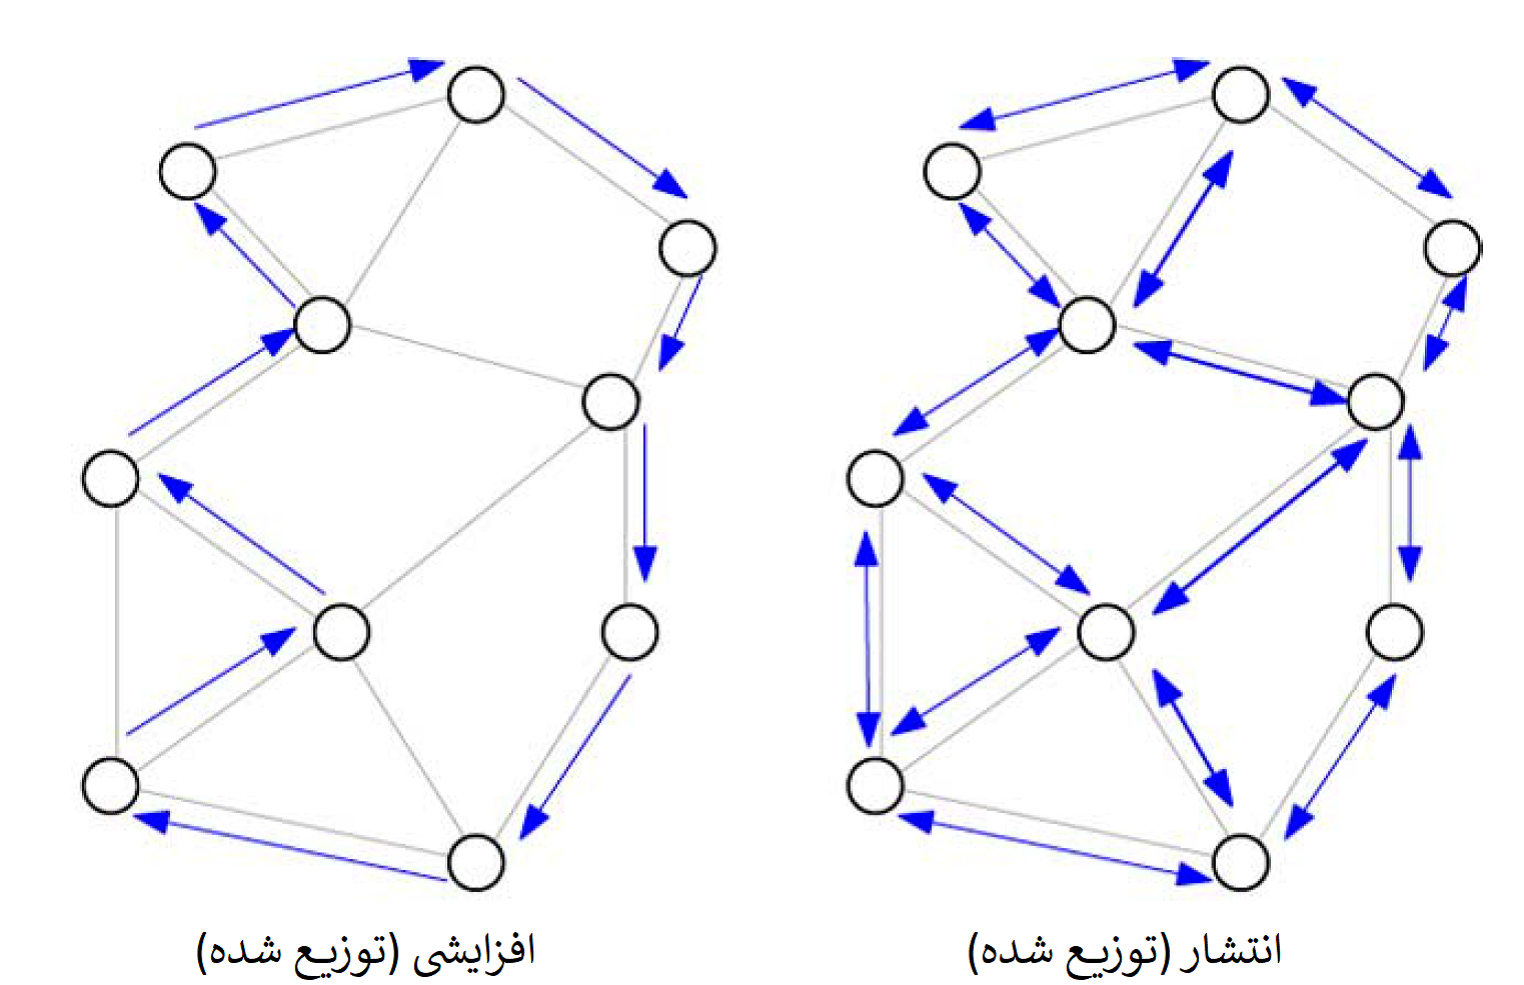
\includegraphics[scale=0.4]{Pic1.png}
		\caption{روش‌های مختلف همکاری بین گره‌ها در یک شبکه توزیع‌شده \cite{Sayed2014} }
		\label{p1}
	\end{center}
\end{figure}

فرض کنید یک شبکه متصل غیرجهت‌‌دار $G(V,E) $ مفروض است که $V$ مجموعه گره‌های شبکه و $E$ مجموعه یال‌های شبکه می‌باشد. گره‌ها در این شبکه تطبیقی با همکاری همدیگر اقدام به حل مساله بهینه‌سازی زیر می‌نمایند:


\begin{equation}\label{e1}
	w_o=\argminA_{w} J^{glob}(w)
\end{equation}

\begin{equation}\label{e2}
	J^{glob}(w)=\frac{1}{N}\sum_{k=1}^{N} J_k(w)
\end{equation}

که $N$ تعداد گره‌های شبکه، $M$ اندازه بردار وزن یا مرتبه فیلتر و $J_k (w)$ تابع زیان محدب و مشتق‌پذیر در گره $k$ام است. $J^{glob} (w)$  تابع زیان سراسری شبکه است که گره‌ها با همکاری همدیگر، پارامتر سراسری $w_o$ را جستجو می‌نمایند. شکل\ref{p2} یک شبکه تطبیقی توزیع‌شده با 12 گره را نشان می‌دهد که هر گره تابع زیان اختصاصی $J_k (w)$ را دارد و تنها با همسایگان خود تبادل اطلاعات انجام می‌دهد. مجموعه $N_k=\{k,l,8,9,N\}$ همسایگان گره \lr{k} را نشان‌می‌دهد که گره $k$ فقط با آنها تبادل داده و همکاری دارد  \cite{Sayed2007}.

\begin{figure}[t!]
	\begin{center}
		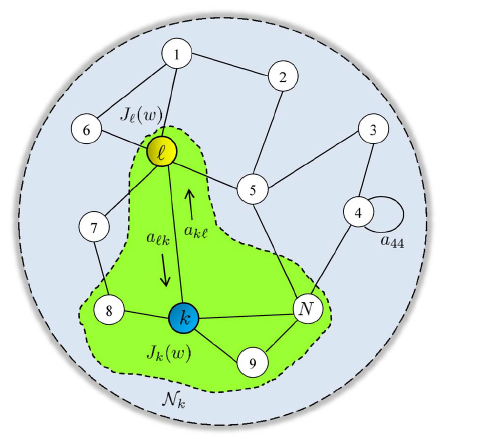
\includegraphics[scale=0.6]{Pic2.png}
		\caption{یک شبکه تطبیقی توزیع‌شده با 12 گره \cite{Sayed2007}}
		\label{p2}
	\end{center}
\end{figure}


اکثر کارهای ارائه‌شده در زمینه برآورد پارامتر از طریق شبکه‌های توزیع‌شده به صورت یک مساله کمینه‌سازی اجماع توابع هزینه هر گره مطرح می‌شوند. گره‌ها با توابع زیان مجزا اما هم مدل در جستجوی یک هدف هستند و نیاز به همگرا شدن به سمت یک پارامتر مشترک دارند. این مسائل تک‌وظیفه‌ای\footnote{\lr{Single Task}} نامیده می‌شوند. دسته دیگر مسائل که هر گره یا گروهی از گره‌ها به دنبال هدف‌هایی مجزا می‌باشند، چند وظیفه‌ای نامیده می‌شوند. 

با فرض داشتن یک شبکه متصل با $N$ گره $(k=1,2,…,N)$، هر گره شبکه در زمان $i$ یک مقدار اسکالر $d_k(i)$ به عنوان سیگنال مطلوب و یک بردار ورودی $u_k (i)\in R^M$ با ماتریس کوواریانس $R_{u,k}=E\{u_k (i),u_k^T (i)\}$ دریافت می‌کند. ورودی‌های هر گره یا مدل داده به صورت زیر با یک رگرسیون خطی مدل می‌شوند:

\begin{equation}\label{e6}
	d_k(i)=u_k^T(i)w^o+\nu_k(i)\qquad i>=0, k=1,2,...,N
\end{equation}

که $w^o$ بردار پارامترها به طول $M$ است و گره‌ها در طی فرآیند یادگیری به دنبال برآورد آن می‌باشند. $z_k (i) $ یک نویز اندازه‌گیری با میانگین صفر و واریانس $\sigma_\nu^2$ می‌باشد. تابع زیان میانگین مربعات خطا (\lr{MSE}) برای هر گره به صورت زیر تعریف می‌شود: 

\begin{equation}\label{e7}
	j_k(w)=E(d_k(i)-u_k^T(i)w)^2
\end{equation}

گره‌ها به دنبال برآورد بردار پارامتر مشترک $w^o$ با استفاده از تابع زیان $J_k (w)$ در شبکه تطبیقی تک‌وظیفه‌ای هستند. شکل \ref{p6} یک شبکه تطبیقی تک وظیفه‌ای را نشان می‌دهد. از آنجایی که تابع زیان در رابطه \ref{e7} یک تابع اکیدا محدب \footnote{\lr{Strongly convex}} است، پس دارای یک مینیمم سراسری $w_k^o$ است. در نتیجه پارامتر $w^o$ در رابطه \ref{e6} همان $w_k^o$ می‌باشد.

\begin{figure}
	\begin{center}
		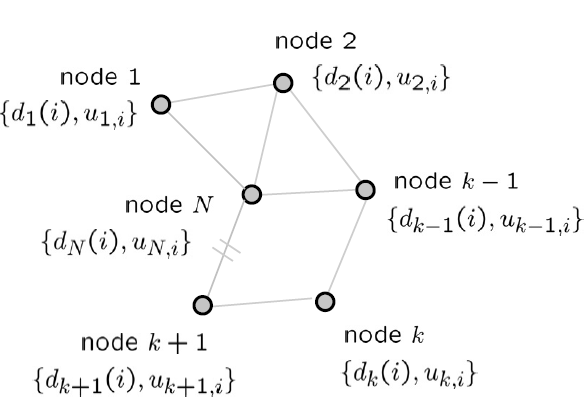
\includegraphics[scale=0.5]{Pic6.png}
		\caption{شبکه تطبیقی تک‌وظیفه‌ای \cite{Bo2010}}
		\label{p6}
	\end{center}
\end{figure}


\section{مدل‌های محاسباتی پردازش موازی و توزیع‌شده}

امروزه با افزایش حجم داده‌های پردازشی و محاسبات سنگین در بسیاری از کاربردها، چالش‌های مهمی در فرآیند یادگیری الگوریتم‌ها مطرح شده است. در یک شبکه تطبیقی توزیع‌شده، اگر عملیات محاسباتی در فرآیند تخمین برای گره‌ها سنگین باشد و یا داد‌های ورودی ذاتاً توزیع‌شده و برای ذخیره در یک گره بسیار بزرگ باشند، مهمترین چالش در این نوع یادگیری، موازی‌سازی فرآیند آموزش و ایجاد یک مدل منسجم در کل شبکه است. یادگیری موازی بهتر است تحت یک مدل یا چارچوب محاسباتی موازی پیاده‌سازی و اجرا شود. در سال‌های اخیر به منظور پردازش‌های موازی و پیاده‌سازی الگوریتم‌های توزیع‌شده مدل‌ها و چارچوب‌های محاسباتی زیادی با ویژگی‌ها و کاربردهای مختلف مورد مطالعه قرار گرفته است. از جمله این مدل‌های محاسباتی می‌توان به \lr{PRAM}، \lr{LogP}، \lr{BSP} و چارچوب \lr{MapReduce} اشاره کرد. 
\subsection{مدل محاسباتی \lr{PRAM}}
مدل محاسباتی \lr{PRAM} (ماشین موازی با دستیابی تصادفی) \cite{Ja1992} یک مدل حافظه اشتراکی است که در آن ارتباط بین پردازنده‌ها از طریق حافظه اشتراکی انجام می‌شود. در صورتی که پردازنده $i$ بخواهد داده‌ای را به پردازنده $j$ ارسال کند، در دو مرحله انجام می‌شود. ابتدا پردازنده $i$ داده را در حافظه مشترک در یک محل شناخته شده برای پردازنده $j$ می‌نویسد و پردازنده $j$ داده را از محل مورد نظر می‌خواند. شکل \ref{P32} مدل محاسباتی \lr{PRAM} را نشان می‌دهد. کامپیوترهای مبتنی بر مدل \lr{PRAM} بر اساس نحوه دسترسی هم‌زمان به یک مکان یکسان به چهار دسته \lr{EREW}، \lr{CREW}، \lr{ERCW} و \lr{CRCW} تقسیم می‌شوند. عمدتاً به این دلیل که هزینه ارتباطات بیشتر از هزینه محاسبات بوده و تعداد پردازنده‌ها محدود می‌باشد، این مدل برای پیاده‌سازی همه‌منظوره در سخت‌افزار مناسب نیست و همچنین منجر به یک مدل برنامه‌نویسی نمی‌شود.
\begin{figure}[t!]
	\begin{center}
		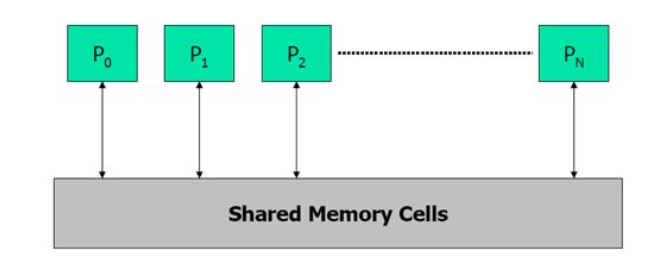
\includegraphics[scale=0.7]{Pram.JPG}
		\caption{مدل محاسباتی\lr{PRAM}\cite{Ja1992} }
		\label{P32}
	\end{center}
\end{figure}

\subsection{مدل محاسباتی \lr{LogP}}
ماشین انتزاعی مدل محاسباتی \lr{LogP} \cite{Logp} شامل تعداد زیادی  پردازنده با حافظه توزیع‌شده است. پردازنده‌ها از طریق یک شبکه ارتباطی انتزاعی به هم متصل می شوند که امکان ارتباط نقطه به نقطه را فراهم می‌کند و به صورت جفتی همگام و به طور کلی غیرهمگام هستند. این مدل با چهار پارامتر زیر توصیف می‌شود:
\begin{itemize}
	\item
	\lr{L}، تأخیر رسانه ارتباطی
	\item
	\lr{o}، هزینه ارسال و دریافت پیام
	\item
	\lr{g}، فاصله مورد نیاز بین دو عملیات ارسال/دریافت. تعبیر رایج تر از این کمیت، معکوس پهنای باند یک کانال ارتباطی پردازنده-پردازنده است
	\item
	\lr{P}، تعداد پردازنده‌ها
\end{itemize}
هر عملیات محلی بر روی هر دستگاه زمان یکسانی را می‌طلبد.  این زمان چرخه پردازنده نامیده می‌شود. شکل \ref{P33} مدل محاسباتی \lr{LogP} و پارامترهای مهم این مدل را به تصویر کشیده است. ارتباطات در این مدل یک نمای محلی بر اساس عملکرد هر جفت پردازنده دارد. 
\begin{figure}[t!]
	\begin{center}
		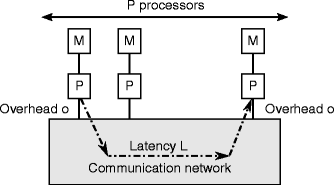
\includegraphics[scale=0.7]{logp.png}
		\caption{مدل محاسباتی\lr{LogP} \cite{LogP2011}}
		\label{P33}
	\end{center}
\end{figure}
\subsection{چارچوب محاسباتی \lr{MapReduce}}
یکی از روش‌های پردازش مجموعه داده‌های عظیم، چارچوب نگاشت-کاهش یا \lr{MapReduce} نام دارد و توجه محققان زیادی را تا کنون به خود جلب کرده است. این چارچوب توسط گوگل\cite{De2008} توسعه یافته و به طور گسترده مورد استفاده قرار گرفته است. اجرای متن باز آن \lr{Hadoop} \cite{Apache58} در حال حاضر توسط بیش از 100 شرکت در سراسر جهان از جمله \lr{eBay}، \lr{IBM}، \lr{Yahoo!}، \lr{Facebook} و \lr{Twitter} و تعدادی از دانشگاه‌ها استفاده می‌شود \cite{Apache59}. برخی از شرکت‌ها مانند آمازون و مایکروسافت به کاربران خود اجازه می‌دهند تا برنامه‌های نگاشت-کاهش را روی ابر خود اجرا کنند \cite{Apache60,Apache61}. الگوریتم‌های نگاشت-کاهش برای حل تعدادی از مسائل غیر پیش پا افتاده در زمینه‌های مختلف از جمله پردازش داده‌ها، داده‌کاوی و تجزیه و تحلیل گراف استفاده شده است.

\lr{Dean}  و همکارش در سال 2004  \cite{De2008} چارچوب محاسبات موازی نگاشت-کاهش را معرفی کردند. ایده اصلی این چهارچوب از زبان‌های مانند \lr{Lisp} گرفته شده است. عمل نگاشت یک تابع و یک دنباله را به عنوان ورودی می‌گیرد و این تابع را بر روی تمام عناصر موجود در دنباله اعمال می‌کند. عمل کاهش، با توجه به یک توالی از مقادیر و یک تابع دودویی، از این تابع برای ترکیب عناصر دنباله‌ در یک مقدار خروجی واحد استفاده می‌کند. دو عمل نگاشت و کاهش در تعدادی دور یا \lr{Round} اجرا می‌شوند و اساس چهارچوب نگاشت-کاهش را تشکیل می‌دهند که در اصل برای اجرا بر روی خوشه‌های بزرگی از ماشین‌های ارزان قیمت طراحی شده‌اند. هر ماشینی یک پردازنده، یک حافظه اولیه سریع و یک حافظه ثانویه کندتر دارد و از طریق یک شبکه زیربنایی به بقیه خوشه متصل است. حافظه ثانویه بخشی از حافظه اشتراکی سراسری است  که هر ماشین تنها در حین همگام‌سازی اجازه دسترسی به حافظه ثانویه ماشین‌های دیگر را دارد. 

داده‌ها در یک الگوریتم نگاشت-کاهش به صورت زوج‌های کلید-مقدار مشخص می‌شوند. همان طور که در شکل\ref{p3} نشان داده شده است، یک الگوریتم نگاشت-کاهش شامل تعدادی دور است که هر دور یک فاز نگاشت و یک فاز کاهش دارد. هر فاز از یک ورودی، یک محاسبات و یک مرحله خروجی تشکیل شده است که خروجی هر فاز به عنوان ورودی فاز بعدی استفاده می‌شود. هنگامی که یک فاز تمام می‌شود، یعنی زمانی که هر ماشین داده‌های خروجی خود را در حافظه اشتراکی می‌نویسد، داده‌ها همگام می‌شوند و هر ماشین اجازه دارد داده‌های نوشته شده در فاز قبلی را بخواند. ماشین‌ها تنها مجاز به برقراری ارتباط با پردازنده اصلی می‌باشند. حافظه اولیه محلی هر ماشین قبل از هر همگام‌سازی به طور کامل پاک می‌شود. در چارچوب نگاشت-کاهش موازی‌سازی از طریق داشتن ماشین‌های مختلف که عملکردهای یکسانی را روی داده‌های مختلف انجام می‌دهند، به دست می‌آید. 
\begin{figure}[t!]
	\begin{center}
		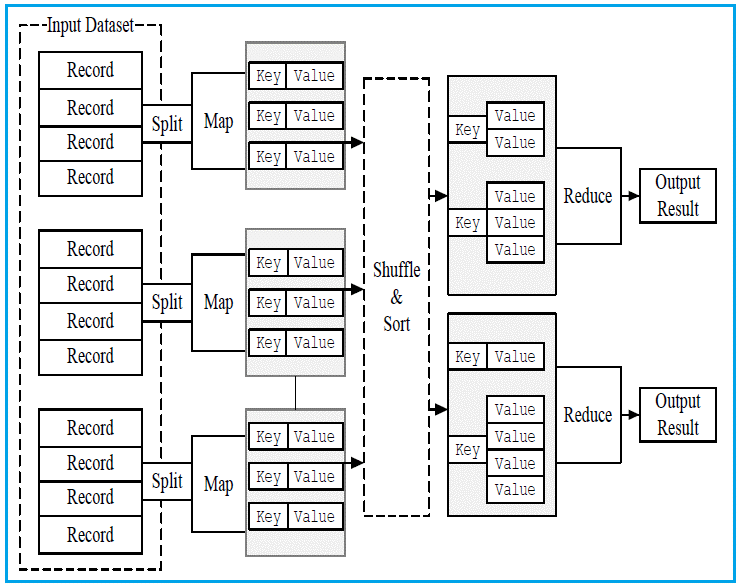
\includegraphics[scale=0.6]{Pic3.png}
		\caption{یک دور در چارچوب نگاشت-کاهش شامل فازهای \lr{Map} و \lr{Reduce} \cite{De2008}}
		\label{p3}
	\end{center}
\end{figure}

\subsection{مدل محاسباتی \lr{BSP}}
مدل محاسباتی \lr{BSP} (موازی‌سازی با همگامی مانعی) \cite{Va1990} تعمیمی از مدل محاسباتی \lr{PRAM} است که توسط پروفسور \lr{L. G. Valiant } از دانشگاه هاروارد در سال 1990 به عنوان یک مدل پل برای محاسبات موازی پیشنهاد شده است. در طی سالهای گذشته این مدل توسط پروفسور \lr{McColl} و \lr{Valiant} توسعه یافته است.  مدل محاسباتی \lr{BSP} شامل بخش‌های زیر می‌باشد:
\begin{itemize}
	\item
	مجموعه‌ای از کامپیوترها که هر یک دارای حافظه محلی می‌باشند
	\item 
	یک شبکه ارتباطی که پیام‌ها را از نقطه‌ای به نقطه دیگر انتقال می‌دهد
	\item 
	مکانیزمی که همگام‌سازی همه یا گروهی از پردازنده‌ها را انجام می‌دهد. 
\end{itemize}
برنامه‌های \lr{BSP} به صورت دنباله‌ای از ابرگام‌ها\footnote{\lr{Superstep}} نوشته می‌شوند. هر ابرگام از سه بخش اصلی تشکیل شده است: محاسبات بر روی داده‌های محلی، ارسال و دریافت پیام به منظور دسترسی به داده‌های غیرمحلی و همگام‌سازی مانعی به منظور تکمیل همه عملیات ارتباطی و از سرگیری محاسبات روی داده‌های محلی یا داده‌هایی که از طریق تبادل پیام به یک پردازنده رسیده‌اند. شکل \ref{p4} بخش‌های مختلف یک ابرگام را به تصویر کشیده است.
\begin{figure}[t!]
	\begin{center}
		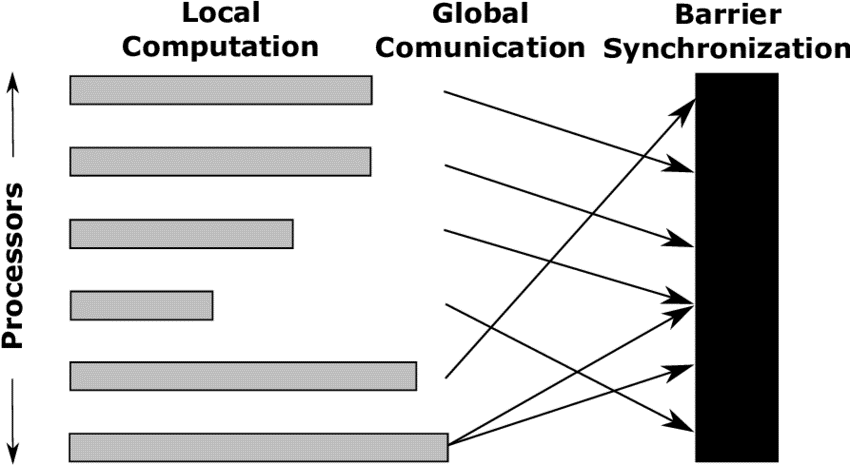
\includegraphics[scale=0.4]{Pic4.png}
		\caption{یک ابرگام در مدل محاسباتی \lr{BSP} \cite{Va1990}}
		\label{p4}
	\end{center}
\end{figure}

یکی از مزیت‌های این مدل محاسباتی این است که می‌توان با استفاده از چهار پارامتر، زمان اجرای یک رویکرد یا الگوریتم طراحی شده بر اساس آن مدل را پیش‌بینی کرد. در بخش \ref{BSP_Dec} به طور مفصل نحوه پیش‌بینی زمان اجرا شرح داده خواهد شد. 

\section{مدل محاسباتی موازی‌ مانعی یا \lr{BSP}}\label{BSP_Dec}

یک کامپیوتر \lr{BSP} شامل مجموعه‌ای از جفت پردازنده-حافظه، یک شبکه ارتباطی کلی و مکانیزمی برای همگام‌سازی مانعی کارآمد پردازنده‌ها است. یک کامپیوتر \lr{BSP} به روش زیر عمل می‌کند. محاسبات شامل دنباله‌ای از ابرگام‌های موازی است، که در آن هر ابرگام متشکل از دنباله‌ای از مراحل است، و به دنبال آن یک همگام‌سازی مانع انجام می‌شود که در آن نقطه، تمام ارتباطات داده تکمیل می‌شوند. در طول یک ابرگام، هر پردازنده می‌تواند تعدادی از مراحل محاسباتی را روی مقادیری که در شروع ابرگام در حافظه محلی‌اش ذخیره می‌شوند، انجام دهد، تعدادی پیام ارسال و دریافت کند، و درخواست‌های مختلف خواندن و نوشتن از راه دور را مدیریت کند\cite{Bisseling2020}.

کامپیوتر \lr{BSP} یک مدل حافظه دو سطحی است، یعنی هر پردازنده ماژول حافظه محلی خود را دارد. تمام حافظه‌های دیگر غیرمحلی هستند و به روشی کارآمد یکنواخت قابل دسترسی می‌باشند. منظور از کارآمدی یکنواخت این است که زمان صرف شده برای خواندن یا نوشتن یک عنصر حافظه غیرمحلی در یک جفت  پردازنده-حافظه دیگر باید مستقل از این باشد که مقدار آن در کدام ماژول حافظه فیزیکی قرار دارد. طراح الگوریتم و برنامه‌نویس نیازی ندارد تا از ساختار حافظه سلسله مراتبی و ساختار خاص شبکه ارتباطی آگاه باشد.

مدل محاسباتی \lr{BSP} هم ساختار افقی (مکانی) و هم ساختار عمودی (زمانی) دارد. ساختار افقی ناشی از همگامی است و از تعداد ثابتی از نخ‌های مجازی تشکیل شده است. در زمان اجرا هر کدام از تردها با یک پردازنده فیزیکی مرتبط هستند. ساختار عمودی از پیشرفت یک محاسبات در طول زمان ناشی می‌شود. در \lr{BSP}، این یک ترکیب متوالی از ابرگام‌های کلی است که به طور مفهومی تمام عرض معماری اجرا را اشغال می‌کند. هر ابرگام به سه مرحله تقسیم می‌شود که شامل موارد زیر می‌باشد:
\begin{itemize}
	\item محاسبات محلی در هر ترد، تنها با استفاده از مقادیر ذخیره شده در حافظه محلی هر پردازنده.
	\item اقدامات ارتباطی، به عنوان مثال. ارسال و دریافت، در میان تردها، شامل انتقال داده‌ها بین پردازنده‌ها
	\item همگام‌سازی مانع، که منتظر می‌ماند تا تمام اقدامات ارتباطی کامل شوند، و سپس داده‌های منتقل شده را در حافظه‌های محلی پردازنده‌های مقصد در دسترس قرار می‌دهد.
\end{itemize}
همجنین می‌توان با استفاده از چهار پارامتر، زمان اجرای یک رویکرد یا الگوریتم طراحی شده بر اساس مدل محاسباتی \lr{BSP} را پیش‌بینی کرد. این چهار پارامتر به صورت زیر تعریف می‌شوند:
\begin{itemize}
	\item $l$: تاخیر شبکه و به معنی کمترین تعداد گام‌های زمانی ممکن بین عملیات همگام‌سازی است
	\item  $p$: تعداد پردازنده‌ها
	\item $s$: سرعت پردازنده‌ها
	\item $g$: نرخ راندمان ارتباطات و به عبارت دیگر تعداد کل عملیات محلی انجام شده به وسیله همه پردازنده‌ها در یک ثانیه تقسیم‌بر تعداد کل کلمات انتقال داده شده توسط شبکه ارتباطی در یک ثانیه است
\end{itemize}

پارامترهای $l=l(p)$ و $g=g(p)$ تابعی از پارامتر $p$ هستند. برای بیان مفهوم این پارامترها باید \lr{h-relation } معرفی شود. \lr{h-relation } یک الگوی ارتباطی سراسری است به این معنا که هر پردازنده می‌تواند حداکثر $h$ واحد داده بفرستد یا دریافت کند. واحدها می‌توانند کلمات یا پیام‌ها باشند. هزینه انجام یک \lr{h-relation } به صورت \lr{gh} تعریف شده است. تعریف هزینه به این صورت بیان می‌شود که فرقی بین فرستادن \lr{m} پیام شامل یک واحد داده یا یک پیام شامل \lr{m } واحد داده وجود ندارد. هزینه هر دو حالت \lr{mgh} است. هزینه یک برنامه \lr{BSP} می‌تواند با استفاده از پارامترهای توصیف‌ شده و برخی اطلاعات اضافی پیش‌بینی شود. هزینه یک ابرگام در محاسبات موازی می‌تواند به صورت زیر بیان شود:

\begin{equation}\label{e4}
	C_s=max{\{w_i\}}+max{\{h_i g\}}+l
\end{equation}

که $C_s$ هزینه ابرگام $s$ و $w_i$ زمان محاسبات پردازنده $i$ در ابرگام $s$ است. $l$ تاخیر شبکه است. پارامتر $h_i$ تعداد واحدهای داده که پردازنده $i$ در طول ابرگام می‌فرستد یا دریافت می‌کند. پارامترهای $w$، $g$ و $l$ باید برحسب سرعت پردازنده بیان شوند. مقادیر $w_i$ و $h_i $ می‌توانند با اندازه‌گیری زمان استفاده شده و تعداد بایت‌های فرستاده شده محاسبه شوند. هزینه‌های یک برنامه \lr{BSP} در $S$ ابرگام شامل $W=\sum_{s=1}^{S}w_s$ و $H=\sum_{s=1}^{S}h_s$ است که در مجموع به صورت زیر بیان می‌شود:
\begin{equation}\label{e5}
	C=W+H.g+S.l
\end{equation}

هزینه یک ابرگام به کندترین پردازنده، بیشترین میزان داده‌ای که یک پردازنده می‌فرستد یا دریافت می‌کند و هزینه همگام‌سازی بستگی دارد. هزینه یک برنامه \lr{BSP } برابر با مجموع هزینه همه ابرگام‌ها در برنامه است \cite{Bisseling2020}. با توجه به فرمول فوق مشخص می‌شود که فاکتورهای مهم در ایجاد و طراحی برنامه‌های \lr{BSP} عبارتند از:
\begin{itemize}
	\item 
	محاسبات در هر ابرگام باید بین پردازنده‌ها متوازن باشد
	\item
	ارتباطات بین همه پردازنده‌ها باید متوازن باشد تا از اختلافات بزرگ $h_i$ اجتناب شود
	\item 
	به دلیل هزینه بالای همگام‌سازی، تعداد ابرگام‌ها باید به حداقل برسد
\end{itemize}

الگوریتم‌ها یا برنامه‌های بالانس‌شده از طریق تقسیم بار محاسباتی و ارتباطی به طور مساوی بین پردازنده‌های در دسترس حاصل خواهند شد. پارامترهای $l$ و $g$ در بین پیاده‌سازی‌های سیستم متغیر هستند. در مقایسه مدل‌های محاسباتی موازی، می‌توان گفت که در مدل \lr{BSP} محاسبات در یک ابرگام می‌توانند زمان‌های متفاوتی داشته باشند و همچنین هزینه‌های ارتباط و همگام‌سازی به صراحت در نظر گرفته شده است، در حالی‌که در مدل \lr{PRAM} این چنین نیست. مدل \lr{PRAM} منجر به یک مدل برنامه‌نویسی نمی‌شود، اما مدل \lr{BSP} دارای یک مدل برنامه‌نویسی است و هیچ محدودیتی بر روی تعداد پردازنده‌ها ندارد. ارتباط در مدل \lr{LogP} یک نمای محلی بر اساس عملکرد هر جفت پردازنده دارد، در حالی‌که ارتباط در مدل \lr{BSP} یک نمای کلی بر اساس عملکرد برای کل برنامه دارد. 

\subsection{تاریخچه مدل محاسباتی \lr{BSP}}
مدل محاسباتی \lr{BSP} در طول دهه 1980 توسط پروفسور \lr{L. Valiant} از دانشگاه هاروارد  توسعه یافته است که مقاله آن در سال 1990  منتشر شد. در بازه 1990 تا 1992، \lr{L. Valiant} و \lr{B. McColl} از دانشگاه آکسفورد در پرینستون و هاروارد روی ایده‌هایی برای مدل برنامه‌نویسی \lr{BSP} حافظه توزیع‌شده کار کردند. در بازه 1992 تا 1997، پروفسور \lr{McColl} یک تیم تحقیقاتی بزرگ را در آکسفورد رهبری کرد که کتابخانه‌ها، زبان‌ها و ابزارهای مختلف برنامه‌نویسی \lr{BSP}، و همچنین الگوریتم‌های موازی متعدد \lr{BSP}، از جمله بسیاری از نمونه‌های اولیه از الگوریتم‌های موازی اجتناب از ارتباط با کارایی بالا و الگوریتم‌های موازی بازگشتی «جاودانه» را توسعه دادند که به بهترین عملکرد ممکن و مبادلات پارامتریک بهینه دست یافتند.

در سال 1996، \lr{McColl} گروهی از آکسفورد، هاروارد، فلوریدا، پرینستون، آزمایشگاه‌های بل، کلمبیا و اوترخت را رهبری کرد که استاندارد \lr{BSPlib} را برای برنامه‌نویسی \lr{BSP} توسعه و منتشر کردند. در دهه 2000، \lr{Valiant} توسعه‌ای برای مدل \lr{BSP} ایجاد کرد که منجر به انتشار مدل \lr{Multi-BSP} در سال 2011 شد \cite{MultiBSP}. 

در سال 2018، پروفسور \lr{McColl} یک تعمیم جدیدی از مدل \lr{BSP} ایجاد کرد که تحمل خطا را برای محاسبات موازی در مقیاس بزرگ در هوش مصنوعی، تجزیه و تحلیل و محاسبات ابری با عملکرد بالا ارائه کرد \cite{BridgingMcColl}.

در سال 2010، گوگل پس از سال‌ها تجربه محدودیت‌های \lr{MapReduce} متوجه شد که به یک مدل جدید برای پشتیبانی از مسائل تحلیلی و محاسباتی گراف‌ها در مقیاس بزرگ نیاز دارند. آنها به سرعت متوجه شدند که با استفاده از مدل \lr{BSP} به روشی داده-محور می‌توانند به اهداف بلندپروازانه‌ای که از نظر مقیاس‌پذیری و عملکرد داشتند، دست یابند. نتیجه سیستم جدید گوگل به نام \lr{Pregel} \cite{Pregle2010} بود که با عبارت جدید "همانند یک راس فکر کن"\footnote{\lr{Think Like a Vertex}} همراه بود \cite{McColl2021}.

در ادامه کار گوگل بر روی \lr{Pregel}، یک سیستم \lr{BSP} منبع-باز داده-محور برای محاسبات گراف به نام \lr{Apache Giraph} توسعه یافت و از آن زمان به بعد چندین سیستم‌ها این چنینی ظاهر شدند. امروزه، \lr{BSP} داده-محور به روشی استاندارد برای انجام محاسبات گراف در مقیاس بزرگ در پایگاه داده‌ها و سایر سیستم‌های تحلیلی، تبدیل شده است.

همانطور که ذکر شد، ایده اصلی پشت سیستم‌های \lr{BSP} داده-محور مانند \lr{Pregel} این است که "مثل راس فکر کنید". این بدان معنی است که ساختار داده، برای مثال، یک گراف با یک میلیارد راس باید به یک محاسبات موازی مجازی نگاشت شود که در آن راس‌ها به محاسبات محلی و یال‌ها به ارتباطات تبدیل می‌شوند. همانند تمام سیستم‌های \lr{BSP}، محاسبات در قالب مجموعه‌ای از دورها یا ابرگام‌ها انجام می‌شود. همانطور که در شکل \ref{BSPDataCenter} نشان داده شده است، در هر دور، هر رأس محاسبات محلی را انجام می‌دهد، پیام‌هایی را به همسایگان خود در گراف ارسال می‌کند و پیام‌هایی را از همسایگان خود دریافت می‌کند. این محاسبات تکراری تا زمانی‌که برخی از شرایط خاتمه برآورد شوند، ادامه می‌یابند \cite{McColl2021}.
\begin{figure}[h]
	\begin{center}
		\includegraphics[scale=0.8]{BSP3step.PNG}
		\caption{\lr{BSP} داده-محور \cite{McColl2021}}
		\label{BSPDataCenter}
	\end{center}
\end{figure} 

در سیستم‌های مبتنی بر \lr{BSP}، ماهیت ابرگام‌ها تضمین می‌کند که هیچ مشکل هم‌زمانی از جمله شرایط مسابقه\footnote{\lr{race conditions}} یا بن‌بست\footnote{\lr{deadlock}} رخ نخواهد داد. البته میزان ریزدانگی موازی بودن مجازی یا منطقی در چنین محاسباتی می‌تواند بسیار زیاد در حد یک میلیارد یا یک تریلیون باشد. از سوی دیگر، ماشین‌های موازی کاربردی معمولاً تنها چند صد یا چند هزار هسته خواهند داشت. بنابراین، همانطور که قبلا ذکر شد، این محاسبات مجازی مقیاس بزرگ را می‌توان به راحتی بر روی یک ماشین موازی فیزیکی در مقیاس بسیار کوچکتر به روشی ساده و سرراست  که ساختار محلی گراف را برای بهینه‌سازی ارتباطات در نظر می‌گیرد، نگاشت کرد.

سیستم‌های \lr{BSP} داده-محور در سال‌های اخیر به طور گسترده توسط بسیاری از شرکت‌ها در سراسر جهان برای محاسبات کاربردی بر روی گراف‌هایی با میلیاردها راس و تریلیون‌ها یال استفاده شده است. علاوه‌بر ارائه مقیاس‌پذیری زیاد و عملکرد بسیار بالا، یادگیری و استفاده از این مدل نیز بسیار آسان است. برای مثال، الگوریتم رتبه‌بندی صفحات \footnote{\lr{PageRank Algorithm}} گوگل که نقش اساسی در روش‌های جستجوی آن‌ها دارد را می‌توان تنها در 15 تا 20 خط کد توصیف کرد، زیرا این الگوریتم را می‌توان در \lr{BSP} داده-محور به‌ صورت محاسبات تکراری ساده زیر فرمول‌بندی کرد:
\begin{enumerate}
	\item خواندن رتبه همسایه‌ها
	\item به‌روزرسانی رتبه محلی
	\item ارسال رتبه جدید به همسایه‌ها
\end{enumerate}

شرکت پایگاه‌داده \lr{TigerGraph} اعلام کرد که پایگاه داده گراف \lr{BSP} داده-محور آن‌ها اکنون سریع‌ترین پایگاه داده گراف تراکنشی در جهان است که حجم عظیمی از تجارت الکترونیک و تراکنش‌های مالی را مدیریت می‌کند. اگرچه در پاراگراف‌های اخیر بیشتر بر مبحث تجزیه و تحلیل گراف با مدل \lr{BSP} داده-محور تاکید شده است، اما در بسیاری از دسته‌های دیگر محاسبات موازی نیز این مدل قابل استفاده است. به عنوان مثال، می‌توان از آن در محاسبات علمی و مهندسی مانند محاسبات شابلون\footnote{\lr{Stencil Computations}}، مسائل \lr{n}-جسم\footnote{\lr{n-body Problems}}، اجزای محدود و مدل‌سازی مدار و همچنین در یادگیری ماشین و سایر زمینه‌های هوش مصنوعی استفاده کرد.


\subsection{برتری‌های مدل محاسباتی \lr{BSP}}
\textbf{همه‌منظوره بودن}

اساس روش \lr{BSP} برای برنامه‌نویسی موازی مفهوم ابرگام است که در آن ارتباطات و همگام‌سازی به طور کامل از هم جدا شده‌اند. یک برنامه \lr{BSP} صرفا برنامه‌ای متشکل از تعدادی فاز است و ارتباطات لازم بین فازها انجام می‌شود. این روش برای برنامه‌نویسی موازی بر روی تمام انواع معماری‌های موازی و الگوریتم‌های موازی قابل اجرا است. این روش یک چارچوب منسجم و بسیار کلی  را برای توسعه نرم‌افزارهای موازی قابل حمل برای معماری‌های موازی مقیاس‌پذیر فراهم می‌کند.

\textbf{سادگی}

برنامه‌های \lr{BSP} تقریبا مشابه برنامه‌های متوالی هستند. تنها اطلاعات اضافی اندکی برای توصیف استفاده از موازی‌سازی باید ارائه شود. 

\textbf{اشکال‌زدایی آسان و بدون بن‌بست}

در حالی‌که ارتباطات و همگام‌سازی در برنامه \lr{BSP} جدا شده‌اند، برنامه‌نویس دیگر لازم نیست نگران مشکلاتی از جمله بن‌بست که می‌تواند با ارسال پیام همگام‌سازی رخ دهد، باشد. به دلیل این جداسازی، اشکال‌زدایی یک برنامه \lr{BSP} بسیار آسان‌تر انجام می‌شود. مانع همگام‌سازی قرار گرفته در انتهای هر ابرگام یک نقطه شکست مناسبی را فراهم می‌کند که در آن حالت کلی محاسبات موازی به خوبی تعریف شده است و می‌تواند مورد بررسی قرار گیرد. بنابراین اشکال‌زدایی و استدلال در مورد درستی یک برنامه \lr{BSP} دشوارتر از یک برنامه متوالی نیست. 

\textbf{قابل حمل بودن و مستقل از معماری هدف}

برخلاف مدل‌های برنامه‌نویسی موازی، \lr{BSP} به صورت یک مدل مستقل از معماری طراحی شده است. بنابراین زمانی‌که برنامه‌ها از یک معماری به معماری دیگری منتقل می‌شوند، بدون نیاز به هیچگونه تغییری اجرا می‌شوند. این امر کاوش فضای طراحی را ممکن می‌سازد، زیرا تأثیر یک تصمیم بر عملکرد به راحتی قابل تعیین است.

\textbf{قابل تجزیه و تحلیل بودن}

مدل هزینه \lr{BSP} روشن می‌کند که چه استراتژی‌هایی باید برای نوشتن برنامه‌های \lr{BSP} کارآمد اتخاذ شود. با توجه به اینکه پارامتر $W$ حداکثر زمان محاسباتی را نشان می‌دهد، باید محاسبات بین رشته‌ها را متعادل و به حداقل رساند. از آنجایی‌که پارامتر $h$ حداکثر داده مبادله شده است، باید ارتباطات بین رشته‌ها را متعادل و به حداقل رساند. تعداد ابرگام‌ها باید به حداقل برسد، زیرا این مورد تعداد دفعاتی که پارامتر $L$ در هزینه نهایی ظاهر می‌شود را تعیین می‌کند. همچنین مدل هزینه چگونگی پیش‌بینی کارآیی روی یک معماری هدف خاص را نشان می‌دهد. مقادیر پارامترهای $W$ و $h$ برای هر ابرگام، و تعداد ابرگام‌ها می‌توانند با بررسی کد برنامه تعیین شوند. با درج مقادیر پارامترهای $p$، $g$ و $L$ می‌توان زمان اجرا را قبل از اجرای برنامه مشخص کرد. 

\textbf{استفاده آسان از نقطه شکست برای انعطاف‌پذیری}

این مورد اشاره دارد به این واقعیت که به راحتی می‌توان یک حالت کاملاً تعریف‌شده را در هر مانع ثبت کرد و یا به عبارت دیگر، یک راه ساده برای انجام بازرسی و بازیابی خرابی‌های سخت‌افزاری است. در مقابل، بررسی وضعیت محاسبات موازی بسیار دشوار است. در مدل محاسباتی \lr{BSP} معنای ابرگام نه تنها امکان مقابله با خرابی‌های سخت‌افزاری را فراهم می‌کند، بلکه به طور مؤثری می‌توان تأخیرهای طولانی را مدیریت کرد، که این خود یک مساله بسیار چالش‌برانگیز است.

\textbf{ارتباطات را می‌توان برای تبادل کلی بهینه کرد}

در محاسبات موازی مقیاس بزرگ، تقریباً همیشه این اتفاق می‌افتد که موازی‌سازی در نرم‌افزار بسیار بیشتر از موازی‌سازی در سخت‌افزار است. این یک نتیجه ساده از قدرت سخت‌افزار محاسباتی مدرن است. در مثالی که یک الگوریتم گراف دارای یک تریلیون کار فرعی موازی است، این وظایف فرعی بر روی یک ماشین فیزیکی که درجه موازی بسیار کمتری دارد، نگاشت می‌شوند. به عنوان مثال، ممکن است روی 200 ماشین 16 هسته‌ای نگاشت شود، در این صورت هر هسته حدود 300 میلیون کار فرعی موازی کوچک را انجام می‌دهد. همان پدیده سستی موازی‌سازی در هر حوزه‌ای از محاسبات موازی در مقیاس بزرگ از جمله محاسبات ماتریس پراکنده، یادگیری ماشین، مدل سازی، بهینه‌سازی و غیره رخ می‌دهد. 

یکی از پیامدهای اصلی سستی موازی‌سازی این است که معمولاً در هر محاسبات موازی در مقیاس بزرگ، هر پردازنده در حین انجام محاسبات با هر پردازنده دیگری ارتباط برقرار می‌کند. بنابراین، برای دستیابی به اوج عملکرد، باید سیستم‌های نرم‌افزاری موازی را طراحی کنیم که برای این الگوی کلی ارتباطات بهینه‌سازی شده باشند و در آن هر پردازنده در حال ارسال به سایرین است و از سایرین دریافت می‌کند. این الگوی ارتباطی، تبادل کل نامیده می‌شود. سیستم‌های نرم‌افزار \lr{BSP} برای تبادل کلی بهینه‌سازی شده‌اند، نه برای ارتباطات زوجی منفرد، مانند \lr{MPI} و سایر سیستم‌های ارسال پیام غیرهمگام یا همگام. زمانی که پردازنده‌ها نیاز به ارسال و دریافت میلیون‌ها مقدار به/از هر پردازنده دیگر در یک دور محاسبات موازی دارند، این امر باعث بهبود قابل توجهی در کارایی و عملکرد می‌شود.

\textbf{ارتباطات می‌تواند غیر مسدودکننده و یک طرفه باشند}

سیستم‌های تبادل پیام همانند \lr{MPI} براساس ارتباطات همگام بین جفت پردازنده‌ها هستند. برای اینکه پردازنده \lr{A} بتواند حتی یک مقدار را به پردازنده \lr{B} ارائه دهد، باید با \lr{B} همگام شود و سپس مقدار را به \lr{B} ارسال کند. این کار از نظر زمانی بسیار پرهزینه است، به خصوص در شرایطی که تعداد زیادی ارتباطات ریز دانه‌ای  وجود دارد که باید اتفاق بیفتد.

در طراحی مدل نرم‌افزار \lr{BSP} و در تعریف استاندارد \lr{BSPlib}، با معرفی ارتباطات یک طرفه بدون کپی غیرمسدودکننده به عنوان مدل پیش فرض ارتباطات، این مساله حل شده است. این به دلیل ساختار ابرگامی محاسبات \lr{BSP}، با مدل همگام‌سازی مانعی آن است. تغییر از ارتباطات آهسته دو طرفه \lr{MPI} به ارتباطات یک طرفه بدون کپی \lr{BSP} منجر به بهبودهای عمده در کارایی و عملکرد مسائل به ویژه برای محاسبات موازی مدرن ریزدانه مانند محاسبات ماتریس پراکنده، جابجایی نمودار و یادگیری ماشین شده است.

در \lr{BSP}، ارتباط داده‌ها را می‌توان با استفاده از \lr{RDMA} \footnote{\lr{Remote Direct Memory Access}} که هم از نظر بازده بالا و هم از نظر تأخیر بسیار کم است، پیاده‌سازی کرد. \lr{RDMA} به سبک \lr{BSP} اکنون مستقیماً در شبکه‌های ارتباطی مانند \lr{InfiniBand} پشتیبانی می‌شود. برخی از نسخه‌های جدیدتر \lr{MPI} موارد اولیه را برای ارتباطات یک طرفه اضافه کرده اند، اگرچه برای استفاده موثر از آنها نیاز به ساختار برنامه \lr{MPI} به سبک \lr{BSP} است.

\textbf{ارتباطات را می‌توان به صورت کلی برنامه‌ریزی و بهینه‌سازی کرد}

در \lr{BSP}، سیستم به طور خودکار ارتباطات و همگام‌سازی را بهینه می‌کند، در حالی که در \lr{MPI} برنامه‌نویس مسئول این بهینه‌سازی است که این کار می‌تواند بسیار پیچیده باشد. یک برنامه‌نویس فوق‌العاده متخصص \lr{MPI} می‌تواند این کار را انجام دهد و با ارتباطات یک طرفه \lr{MPI-2} ممکن است در برخی موارد بتواند به عملکرد قابل مقایسه با \lr{BSP} دست یابد. با این حال، با استفاده از ابزارهای \lr{BSP} به طور مستقیم، این پیچیدگی از کار برنامه‌نویس حذف می‌شود و سیستم می‌تواند به طور خودکار ارتباطات را برای اطمینان از حداکثر توان شبکه و تأخیر بسیار کم، با حذف تراکم، برنامه‌ریزی کند. این موارد در \lr{BSP} امکان‌پذیر است زیرا ارتباطات غیر مسدودکننده و به هر ترتیبی است. سیستم می‌تواند تبادل کل پیام‌ها بین گره‌ها را برنامه‌ریزی کند تا اطمینان حاصل شود که شبکه در تمام نقاط دارای بار متعادل است.

\subsection{کتابخانه‌‌های نرم‌افزاری برای مدل محاسباتی \lr{BSP} }
مدل محاسباتی \lr{BSP} می‌تواند به عنوان چارچوبی برای برنامه‌نویسی با کارایی بالا در نظر گرفته شود که به طور خاص سعی می‌کند دو مساله زیر را حل نماید:
\begin{itemize}
	\item 
	امکان شرایط مسابقه: جایی‌که پردازنده دیگری به طور نامطلوب حافظه را در طول اجرای کد تغییر می‌دهد.
	\item
	امکان شرایط بن‌بست: جایی که یک چرخه به صورت انتظار پردازنده-1 برای پردازنده-2، انتظار پردازنده-1 برای پردازنده-3 و غیره شکل می‌گیرد.
\end{itemize}
مدل \lr{BSP} این مسائل را با جداسازی کامل ارتباط بین پردازنده‌ها از محاسبات درون یک پردازنده حل می‌کند. به عبارت دیگر، پردازنده‌ها هر دوی این عملیات را به صورت \lr{Bulk} انجام می‌دهند. علاوه‌بر این، مدل \lr{BSP} این محدودیت را اضافه می‌کند که هر پردازنده باید در هر نقطه از زمان در یک نوع عملکرد یکسان باشد. به عبارت دیگر، پردازنده‌ها باید هماهنگ باشند که این امر با افزودن موانع  به برنامه دست می‌یابد. موانع دستوراتی هستند که هر پردازنده باید قبل از اجازه داشتن به ادامه کار به آنها برسد. فضای بین این موانع معمولاً به عنوان یک ابرگام  شناخته می‌شود و در 2 مدل ارتباطی یا محاسباتی وجود دارد.  
فرض کنید که یک برنامه \lr{BSP} را روی 5 هسته یا پردازنده اجرا می‌کنیم. شکل \ref{P34} نموداری از اجرای آن نشان می‌دهد که در آن زمان از بالا به پایین اجرا می‌شود و نوارهای خاکستری روشن زمان صرف‌شده برای انجام محاسبات و فلش‌ها ارتباطات را نشان می‌دهند. نوارهای افقی تیره موانعی را نشان می‌دهد که در آن همه پردازنده‌ها هماهنگ می‌شوند.

\begin{figure}[t!]
	\begin{center}
		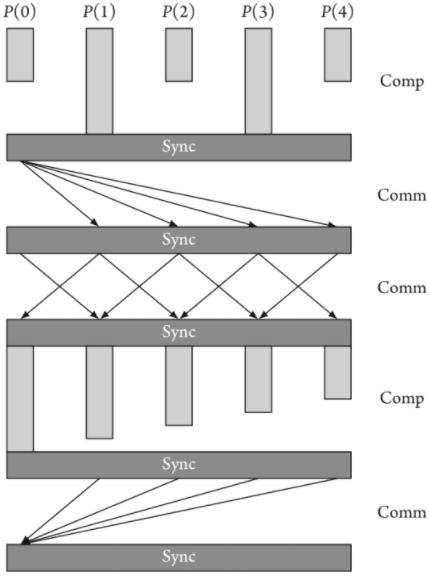
\includegraphics[scale=0.4]{Pic34.png}
		\caption{یک فرآیند \lr{BSP} با 5 ابرگام}
		\label{P34}
	\end{center}
\end{figure}

در شکل \ref{P34} یک فرآیند \lr{BSP} نشان داده شده است که در مجموع برای 5 مرحله ابرگام اجرا شده است. پردازنده‌های 0، 2 و 4 در مرحله اول، فقط به اندازه نصف پردازنده‌های 1 و 3 محاسبه انجام می‌دهند. بنابراین باید 50 درصد مواقع بیکار بمانند. این نکته مهم که در برنامه‌نویسی موازی به ویژه برنامه‌نویسی موازی از طریق \lr{BSP} برجسته است همان اطمینان از متعادل بودن بار محاسباتی بین پردازنده‌ها است. در ادامه کتابخانه‌‌هایی که مدل محاسباتی \lr{BSP} را پشتیبانی می‌کنند و امکانات آنها به طور مختصر آورده شده است.

کتابخانه نرم‌افزاری \lr{BSPy} در زبان برنامه‌نویسی پایتون عملکردهای کلیدی زیر را پشتیبانی می‌کند: 
\begin{itemize}
	\item 
	\lr{bsp.cores()}: درخواست تعداد کل پردازنده‌هایی که به صورت موازی کار می‌کنند
	\item
	\lr{bsp.pid}: درخواست شناسه پردازنده جاری   
	\item 
	\lr{bsp.send()}: ارسال پیام از این پردازنده به دیگری
	\item 
	\lr{bsp.move()}: انتقال پیام به خارج از صف «پیام‌های دریافت‌شده»
	\item 
	\lr{bsp.sync()}: شروع یک ابرگام جدید با همگام‌سازی همه پردازنده‌ها
\end{itemize}

کتابخانه نرم‌افزار دیگری وجود دارد که برای این منظور طراحی شده است و بسیار ساده است. کتابخانه \lr{BSPlib} از 20 نمونه اولیه تشکیل شده است که عملکرد و سرعت مشابه‌ای با \lr{MPI} ارائه می‌دهند. این کتابخانه امکان  ایجاد برنامه‌های موازی را مطابق با الگوی برنامه‌نویسی \lr{BSP} فراهم می‌کند و این امکان را می‌دهد که یک الگوریتم موازی را به شیوه‌ای بسیار ساختاریافته برنامه‌ریزی کرد و در نتیجه کدی خوانا و سریع بدست آورد. \lr{BSPlib} قبلاً برای چندین ابرکامپیوتر و کلاسترهایی از رایانه‌های شخصی پیاده‌سازی شده است، اما از آنجایی که محبوبیت کمتری نسبت به \lr{MPI} دارد، برای همه پلتفرم‌های سخت‌افزاری پیاده‌سازی نشده است. از آنجایی که مهندسان و ریاضیدانان همیشه بالاترین درصد توان محاسباتی را می‌خواهند، در نتیجه اجرای کارآمد یک برنامه مبتنی بر \lr{MPI} ضروری می‌باشد. در حال حاضر دو پیاده‌سازی اصلی از \lr{BSPlib} شامل \lr{Oxford BSP Toolset} و \lr{PUB} وجود دارد که برای پلتفرم‌های سخت‌افزاری خاص (\lr{Cray T3E} یا \lr{SGI Origin} و غیره) پیاده‌سازی شده‌اند. معماری کتابخانه نرم‌افزاری آنها برای استفاده از ویژگی‌های خاص سخت‌افزار بهینه شده است. بنابراین اگر سخت‌افزار/نرم‌افزار توسط یکی از این دو کتابخانه پشتیبانی نشود، باید از \lr{BSPonMPI} در ترکیب با کتابخانه \lr{MPI} استفاده کرد که بسیار سریع است. 

کتابخانه \lr{BSPonMPI} یک کتابخانه نرم‌افزاری مستقل برای توسعه برنامه‌های موازی به زبان برنامه‌نویسی \lr{C} است که استاندارد \lr{BSPlib}\cite{BSPLib} را پیاده‌سازی می‌کند و روی همه ماشین‌هایی که دارای \lr{MPI} هستند، اجرا می‌شود. این ویژگی اصلی این کتابخانه است که آن را از سایر کتابخانه‌ها مانند \lr{Oxford BSP Toolset} و \lr{PUB}\cite{PUB1,PUB2}\footnote{\lr{Paderborn University BSP }} متمایز می‌کند. \lr{MPI} یا \lr{Message Passing Interface} یک \lr{API} برای برنامه‌نویسی موازی می‌باشد که باید نوشتن یک برنامه موازی را آسان کند اما در عمل بسیار پیچیده است، زیرا این \lr{API} شامل صدها تابع می‌باشد. همچنین در حین برنامه‌نویسی موازی بر اساس \lr{MPI} باید مراقب بود که از خطاهای برنامه‌نویسی موازی معمولی مانند بن‌بست یا رفتار نامعین اجتناب شود. 

کتابخانه \lr{PyBSP} یک کتابخانه نرم‌افزاری برای توسعه محاسبات موازی \lr{BSP} است که هدف آن پشتیبانی از \lr{BSP} در پایتون با یک ماژول بسیار ساده پایتونی به نام \lr{bsp} می‌باشد. با استفاده از توابع موجود در این کتابخانه می‌توان پایتون را به یک \lr{BSP} واقعی تبدیل کرد. برخی از این توابع به شرح زیر می‌باشد:
\begin{itemize}
	\item 
	\lr{bsp.procCount()}: تعداد کل پردازنده‌ها را مشخص می‌کند
	\item 
	\lr{bsp.myProcID()}: شماره پردازنده جاری را مشخص می‌کند
	\item 
	\lr{bsp.fromObject(somePythonObject, 'name1')}: داده‌ها باید قبل از ارسال به سایر پردازنده‌ها بسته‌بندی شوند. با این دستور محتوای یک شی بسته‌بندی شده و بسته  \lr{"name1"} نامگذاری می‌شود.
	\item 
	\lr{bsp.fromNumpy(someNumpyArray, 'name2')}: این دستور محتوای یک آرایه \lr{numpy} را بسته‌بندی می‌کند و بسته  \lr{"name2"} نامگذاری می‌شود.
	\item 
	\lr{bsp.toProc(someProcID, 'name1')}: ارسال بسته \lr{"name1"} به پردازنده با شناسه‌ \lr{someProcID}
	\item 
	\lr{bsp.sync('some pass phrase')}:	دستور همگام‌سازی کلی برای شروع تبادل داده و منتظر ماندن برای آن است. عبارت \lr{'some pass phrase'} برای جلوگیری از همگام‌سازی‌های مختلف به یکدیگر است.
\end{itemize}

پکیج \lr{ScientificPython} مجموعه‌ای از ماژول‌های پایتون است که برای محاسبات علمی مفید است. در این مجموعه ماژول‌هایی برای هندسه پایه (بردارها، تانسورها، تبدیل‌ها، میدان‌های برداری و تانسوری)، کواترنیون‌ها، مشتقات خودکار، درون‌یابی (خطی)، چند جمله‌ای‌ها، آمار ابتدایی، برازش‌های حداقل مربعات غیرخطی، محاسبات واحد، فرترن- قالب‌بندی متن سازگار، تجسم سه‌بعدی از طریق \lr{VRML}، و دو ویجت \lr{Tk} برای نمودارهای خط ساده و مدل‌های قاب سیمی سه‌بعدی وجود دارد. همچنین رابط‌هایی برای کتابخانه\lr{MPI} (واسط ارسال پیام، برنامه‌نویسی موازی مبتنی بر پیام) و \lr{BSPlib} (برنامه‌نویسی موازی همگام مانعی) وجود دارد. اکوسیستم علمی پایتون بدون حفظ سازگاری با نسخه‌های قدیمی‌تر، با سرعتی سریع در حال تغییر است. از آغاز توسعه \lr{ScientificPython} در سال 1995، تغییرات مهمی در خود زبان پایتون بین \lr{Python 2.7} و \lr{Python 3} و همچنین تعداد زیادی تغییرات ناسازگار کوچکتر در کتابخانه \lr{NumPy} که \lr{ScientificPython} به آن وابسته است، رخ داده است که این پکیج با این تغییرات سازگار نیست. بنابراین \lr{ScientificPython} فقط با \lr{Python 2.7} و \lr{NumPy 1.8} قابل استفاده است.


\section{خلاصه}
در این فصل، مروری بر مفاهیم اولیه مورد نیاز در زمینه شبکه‌های تطبیقی توزیع‌شده و مدل‌های محاسباتی موازی برای درک بهتر مطالب این رساله ارائه شد. همچنین تاریخچه و برتری‌های مدل محاسباتی موازی‌سازی مانعی و امکانات نرم‌افزاری فراهم شده برای آن ارائه گردید. در ادامه در فصل آینده، کارهای پیشین و مرتبط به این رساله مطرح خواهند شد. 









